\section{\textit{Backstory}}

Cristiano Ronaldo dos Santos Aveiro sedang berencana mengekspansi bisnisnya ke bidang hospitalitas dan ingin membuat sebuah penginapan. Sebagai salah satu pendukung dan penggemar terbesar Lab AI ‘ (eMudhra$^2$ + CR$\bigcirc$) STEI ITB, Cristiano Ronaldo meminta tolong kepada kami, para asisten, untuk membantunya membuat sistem cerdas untuk dapat mengestimasi pengunjung yang akan membatalkan pesanannya agar penginapannya dapat memiliki gambaran yang lebih akurat. Ronaldo Hotel\textsuperscript{TM} akan menggunakan sistem dengan pembelajaran mesin klasik untuk mendapatkan kinerja yang baik tanpa sumber daya komputasi yang besar seperti \textit{Deep Learning}.

Karena Lab AI 23 sedang sibuk menyelamatkan dunia dari bahaya intergalaktik dan harus bekerja dalam bayang-bayang, kami akan menyerahkan tugas ini ke member akademi La Fabrica (kalian). Oleh karena itu, bantulah “GOAT no debat \#earnednotgiven”, para asisten Lab AI, untuk mengerjakan permintaan Ronaldo dengan baik.

\begin{figure}[H]
    \centering
    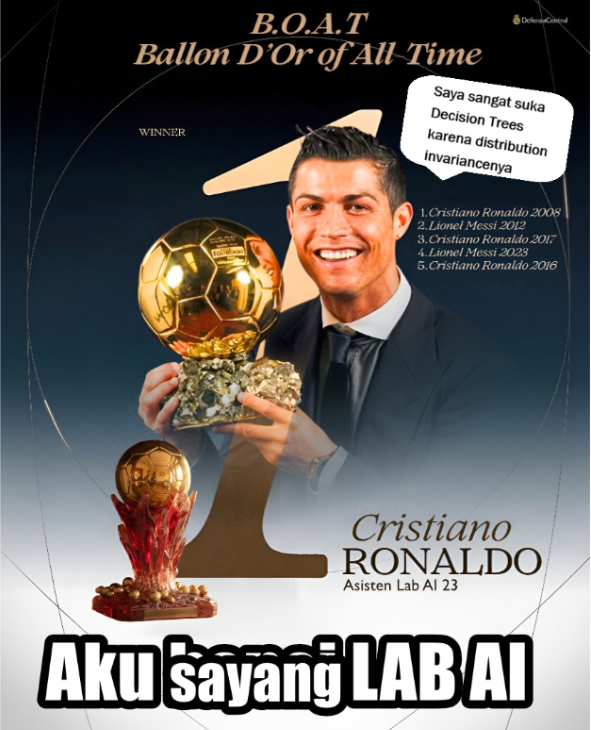
\includegraphics[width=0.5\textwidth]{backstory.png}
    \caption{Ilustrasi konteks pengelolaan pemesanan di Ronaldo Hotel.}
\end{figure}

\section{\textit{Overview} Permasalahan}

Penelitian ini mengkaji prediksi pembatalan pemesanan pada penginapan. Pembatalan yang diketahui lebih awal dapat membantu pengelola memperkirakan ketersediaan kamar dan merencanakan tindakan seperti pengingat kepada tamu, kebijakan pembatalan, atau strategi pemesanan kamar. Sistem yang dikembangkan ditujukan untuk membantu Ronaldo Hotel memperkirakan apakah suatu pemesanan akan dibatalkan.

Data pemesanan memuat beragam karakteristik, antara lain informasi tamu dan lama menginap, paket makanan, kategori kamar, kanal pemesanan, harga, serta riwayat pemesanan. Fitur-fitur tersebut terdiri atas data numerik dan kategorikal sehingga perlu dipahami dan disiapkan agar dapat digunakan oleh algoritma klasifikasi. Target prediksi bersifat biner dengan nilai 1 untuk pemesanan yang dibatalkan dan nilai 0 untuk pemesanan yang tidak dibatalkan.

Permasalahan ini dirumuskan sebagai klasifikasi terawasi. Tugas meminta implementasi beberapa algoritma pembelajaran mesin klasik dari nol, termasuk K-Nearest Neighbors, Decision Tree Learning, Logistic Regression, Support Vector Machine, dan Naive Bayes, kemudian membandingkan hasilnya dengan implementasi scikit-learn. Evaluasi menggunakan Macro F1 agar kinerja prediksi pada kelas pemesanan batal dan tidak batal diperhitungkan secara seimbang.
